%%%%%%%%%%%%%%%%%%%%%%%%%%%%%%%%%%%%%%%%%
% Large Colored Title Article
% LaTeX Template
% Version 1.1 (25/11/12)
%
% This template has been downloaded from:
% http://www.LaTeXTemplates.com
%
% Original author:
% Frits Wenneker (http://www.howtotex.com)
%
% License:
% CC BY-NC-SA 3.0 (http://creativecommons.org/licenses/by-nc-sa/3.0/)
%
%%%%%%%%%%%%%%%%%%%%%%%%%%%%%%%%%%%%%%%%%

%----------------------------------------------------------------------------------------
%	PACKAGES AND OTHER DOCUMENT CONFIGURATIONS
%----------------------------------------------------------------------------------------

\documentclass[paper=a4, fontsize=11pt, onecolumn]{scrartcl}	 % A4 paper and 11pt font size

\usepackage{lipsum} % Used for inserting dummy 'Lorem ipsum' text into the template
\usepackage[english]{babel} % English language/hyphenation
\usepackage[protrusion=true,expansion=true]{microtype} % Better typography
\usepackage{amsmath,amsfonts,amsthm} % Math packages
\usepackage[svgnames]{xcolor} % Enabling colors by their 'svgnames'
\usepackage[hang, small,labelfont=bf,up,textfont=it,up]{caption} % Custom captions under/above floats in tables or figures
\usepackage{booktabs} % Horizontal rules in tables
\usepackage{fix-cm}	 % Custom font sizes - used for the initial letter in the document
\usepackage{graphicx}

\usepackage{sectsty} % Enables custom section titles
\allsectionsfont{\usefont{OT1}{phv}{b}{n}} % Change the font of all section commands

\usepackage{fancyhdr} % Needed to define custom headers/footers
\pagestyle{fancy} % Enables the custom headers/footers
\usepackage{lastpage} % Used to determine the number of pages in the document (for "Page X of Total")

% Headers - all currently empty
\lhead{}
\chead{}
\rhead{}

% Footers
\lfoot{}
\cfoot{}
\rfoot{\footnotesize Page \thepage\ of \pageref{LastPage}} % "Page 1 of 2"

\renewcommand{\headrulewidth}{0.0pt} % No header rule
\renewcommand{\footrulewidth}{0.4pt} % Thin footer rule

\usepackage{lettrine} % Package to accentuate the first letter of the text
\newcommand{\initial}[1]{ % Defines the command and style for the first letter
\lettrine[lines=3,lhang=0.3,nindent=0em]{
\color{DarkGoldenrod}
{\textsf{#1}}}{}}

%----------------------------------------------------------------------------------------
%	TITLE SECTION
%----------------------------------------------------------------------------------------

\usepackage{titling} % Allows custom title configuration

\newcommand{\HorRule}{\color{DarkGoldenrod} \rule{\linewidth}{1pt}} % Defines the gold horizontal rule around the title

\pretitle{\vspace{-30pt} \begin{flushleft} \HorRule \fontsize{40}{40} \usefont{OT1}{phv}{b}{n} \color{DarkRed} \selectfont} % Horizontal rule before the title

\title{AM Modulation} % Your article title

\posttitle{\par\end{flushleft}\vskip 0.5em} % Whitespace under the title

\preauthor{\begin{flushleft}\large \lineskip 0.5em \usefont{OT1}{phv}{b}{sl} \color{DarkRed}} % Author font configuration

\author{Ali Alipour Fereidani, } % Your name

\postauthor{\footnotesize \usefont{OT1}{phv}{m}{sl} \color{Black} % Configuration for the institution name
University of Tehran % Your institution

\par\end{flushleft}\HorRule} % Horizontal rule after the title

\date{} % Add a date here if you would like one to appear underneath the title block

%----------------------------------------------------------------------------------------

\begin{document}

\maketitle % Print the title

\thispagestyle{fancy} % Enabling the custom headers/footers for the first page 

%----------------------------------------------------------------------------------------
%	ABSTRACT
%----------------------------------------------------------------------------------------

%----------------------------------------------------------------------------------------
%	ARTICLE CONTENTS
%----------------------------------------------------------------------------------------

\section*{Introduction}
Amplitude Modulation (AM) is a fundamental modulation technique used in various communication systems. It operates by varying the amplitude of a high-frequency carrier wave in proportion 
to the amplitude of a lower-frequency modulating signal, which contains the information to be transmitted. This report explores AM's principles and components based on the provided technical documentation.

\section*{Technical Details from the Document}

\subsection*{Mathematical Representation}
The document highlights key signals involved in AM:
\begin{itemize}
    \item \textbf{Carrier Signal:} Represented as \( \cos(2\pi f_c t) \), where \( f_c = 430 \, \text{kHz} \).
    \item \textbf{Modulating Signal:} Represented as \( \cos(2\pi f_m t) \), with \( f_m = 94 \, \text{Hz} \).
\end{itemize}

The modulated signal can be expressed as:
\[
s(t) = A_c \left[1 + m(t)\right] \cos(2\pi f_c t)
\]
Here:
\begin{itemize}
    \item \( A_c \): Amplitude of the carrier wave.
    \item \( m(t) \): Modulating signal normalized to avoid overmodulation.
\end{itemize}

Figure 1 illustrates the block diagram of this transformation.

\begin{figure}[ht]
    \centering
  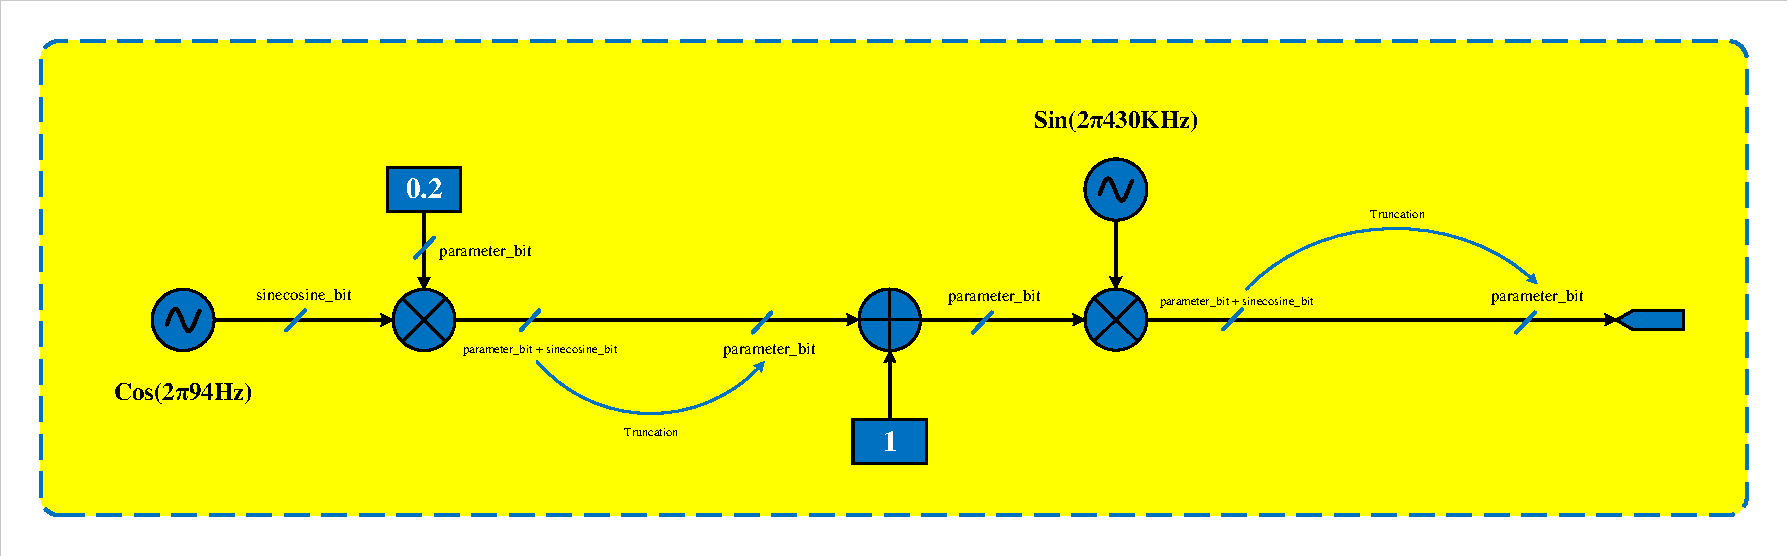
\includegraphics[width=0.8\textwidth]{AM_Modulation.pdf}
  \caption{Block Diagram of the AM Modulation Process}
  \label{fig:Block}
\end{figure}

\subsection*{Parameter Bits and Sine/Cosine Bits}
The document introduces two important concepts related to digital representations in AM:
\begin{itemize}
    \item \textbf{Parameter\_Bit:} Represents the number of constant bits used for amplitude representation.
    \item \textbf{SineCosine\_Bit:} Represents the number of bits used for the output of sine and cosine functions in digital modulation.
\end{itemize}

\subsection*{Truncation Techniques}
Truncation is referenced multiple times, indicating a process to limit the number of bits used in signal representation. This step is essential for balancing precision and computational 
efficiency in digital implementations of AM.

\section*{Analysis of the AM Implementation}

\subsection*{Frequency Characteristics}
The document specifies distinct frequency components:
\begin{itemize}
    \item A carrier frequency of 430 kHz, suitable for medium-wave transmissions.
    \item A modulating frequency of 94 Hz, indicative of a low-frequency audio signal.
\end{itemize}

These values align with typical AM applications in radio broadcasting, where the carrier frequency is significantly higher than the modulating signal to ensure efficient transmission.

\subsection*{Bit-Level Modulation}
Using bit-level operations for parameter and sine/cosine values indicates a focus on digital AM implementations. By managing bit precision, the system optimizes hardware performance while 
minimizing distortion.

\subsection*{Truncation and Signal Processing}
Truncation impacts signal quality by reducing the number of bits representing critical parameters. This approach balances the trade-off between resource efficiency and fidelity, crucial 
in embedded systems and digital communication.

\section*{Applications and Relevance}
\begin{enumerate}
    \item \textbf{Radio Broadcasting:} AM is widely used for commercial radio, where low-frequency audio signals are transmitted over long distances.
    \item \textbf{Digital Signal Processing:} The document's focus on truncation and bit-level operations is relevant for implementing AM in microcontroller-based systems.
    \item \textbf{Education and Research:} Detailed exploration of AM techniques aids in understanding foundational communication principles.
\end{enumerate}

\section*{Result}
The simulation results of this transformation are presented in Figure 2.
\begin{figure}[ht]
    \centering
  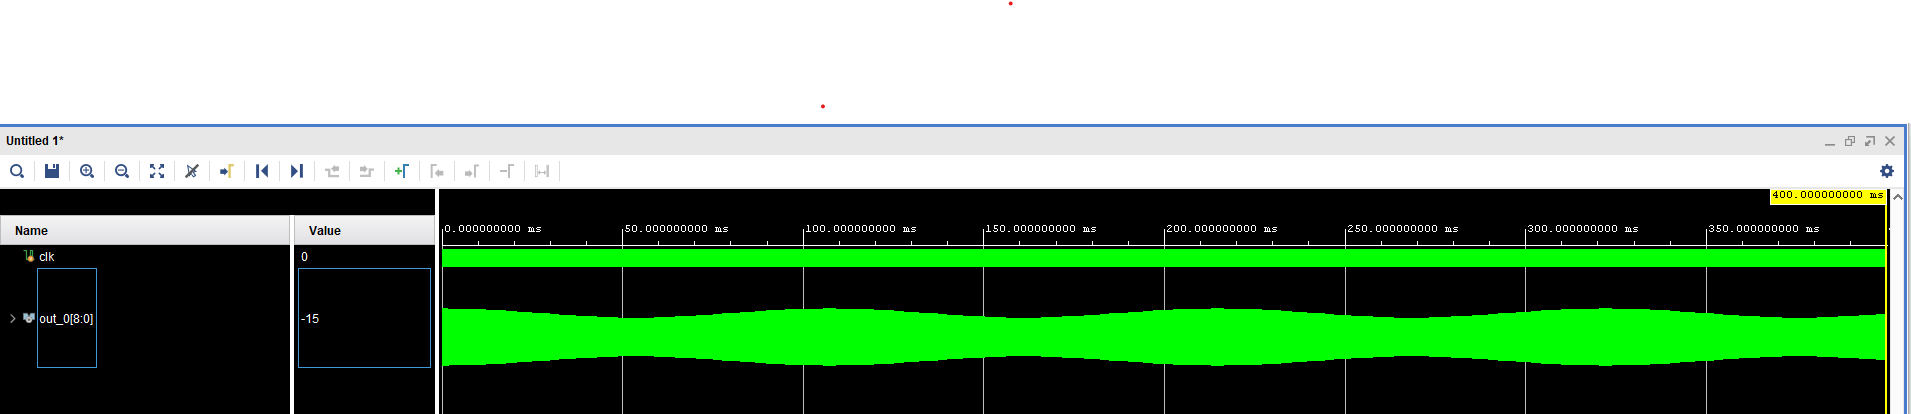
\includegraphics[width=0.8\textwidth]{C:\\Users\\USER\\Documents\\Vivado_pro\\Session_4\\AM Modulation\\Image\\Result.png}
  \caption{Simulation Result}
  \label{fig:Result}
\end{figure}


\section*{Conclusion}
The document provides a detailed exploration of amplitude modulation, emphasizing the mathematical basis, frequency characteristics, and digital signal processing techniques. 
Key concepts such as truncation, parameter bits, and sinecosine bits illustrate the practical challenges and solutions in modern AM implementations. These insights are invaluable 
for applications ranging from broadcasting to digital communication system design.

% \lipsum[1-3] % Dummy text

% \begin{align}
% A = 
% \begin{bmatrix}
% A_{11} & A_{21} \\
% A_{21} & A_{22}
% \end{bmatrix}
% \end{align}


% \lipsum[4] % Dummy text

%------------------------------------------------

% \subsection*{Subsection 1}

% \lipsum[5] % Dummy text

% \begin{itemize}
% \item First item in a list 
% \item Second item in a list 
% \item Third item in a list
% \end{itemize}

% \lipsum[6] % Dummy text

%------------------------------------------------

% \subsection*{Subsection 2}

% \lipsum[7] % Dummy text

% \begin{table}
% \caption{Random table}
% \centering
% \begin{tabular}{llr}
% \toprule
% \multicolumn{2}{c}{Name} \\
% \cmidrule(r){1-2}
% First name & Last Name & Grade \\
% \midrule
% John & Doe & $7.5$ \\
% Richard & Miles & $2$ \\
% \bottomrule
% \end{tabular}
% \end{table}

% %------------------------------------------------

% \section*{Section 2}

% \lipsum[8] % Dummy text

% \begin{description}
% \item[First] This is the first item
% \item[Last] This is the last item
% \end{description}

% \lipsum[9] % Dummy text

%----------------------------------------------------------------------------------------
%	REFERENCE LIST
%----------------------------------------------------------------------------------------

% \begin{thebibliography}{99} % Bibliography - this is intentionally simple in this template

% \bibitem[Figueredo and Wolf, 2009]{Figueredo:2009dg}
% Figueredo, A.~J. and Wolf, P. S.~A. (2009).
% \newblock Assortative pairing and life history strategy - a cross-cultural
%   study.
% \newblock {\em Human Nature}, 20:317--330.
 
% \end{thebibliography}

%----------------------------------------------------------------------------------------

\end{document}